\documentclass{article}\usepackage[]{graphicx}\usepackage[]{color}
% maxwidth is the original width if it is less than linewidth
% otherwise use linewidth (to make sure the graphics do not exceed the margin)
\makeatletter
\def\maxwidth{ %
  \ifdim\Gin@nat@width>\linewidth
    \linewidth
  \else
    \Gin@nat@width
  \fi
}
\makeatother

\definecolor{fgcolor}{rgb}{0.345, 0.345, 0.345}
\newcommand{\hlnum}[1]{\textcolor[rgb]{0.686,0.059,0.569}{#1}}%
\newcommand{\hlstr}[1]{\textcolor[rgb]{0.192,0.494,0.8}{#1}}%
\newcommand{\hlcom}[1]{\textcolor[rgb]{0.678,0.584,0.686}{\textit{#1}}}%
\newcommand{\hlopt}[1]{\textcolor[rgb]{0,0,0}{#1}}%
\newcommand{\hlstd}[1]{\textcolor[rgb]{0.345,0.345,0.345}{#1}}%
\newcommand{\hlkwa}[1]{\textcolor[rgb]{0.161,0.373,0.58}{\textbf{#1}}}%
\newcommand{\hlkwb}[1]{\textcolor[rgb]{0.69,0.353,0.396}{#1}}%
\newcommand{\hlkwc}[1]{\textcolor[rgb]{0.333,0.667,0.333}{#1}}%
\newcommand{\hlkwd}[1]{\textcolor[rgb]{0.737,0.353,0.396}{\textbf{#1}}}%
\let\hlipl\hlkwb

\usepackage{framed}
\makeatletter
\newenvironment{kframe}{%
 \def\at@end@of@kframe{}%
 \ifinner\ifhmode%
  \def\at@end@of@kframe{\end{minipage}}%
  \begin{minipage}{\columnwidth}%
 \fi\fi%
 \def\FrameCommand##1{\hskip\@totalleftmargin \hskip-\fboxsep
 \colorbox{shadecolor}{##1}\hskip-\fboxsep
     % There is no \\@totalrightmargin, so:
     \hskip-\linewidth \hskip-\@totalleftmargin \hskip\columnwidth}%
 \MakeFramed {\advance\hsize-\width
   \@totalleftmargin\z@ \linewidth\hsize
   \@setminipage}}%
 {\par\unskip\endMakeFramed%
 \at@end@of@kframe}
\makeatother

\definecolor{shadecolor}{rgb}{.97, .97, .97}
\definecolor{messagecolor}{rgb}{0, 0, 0}
\definecolor{warningcolor}{rgb}{1, 0, 1}
\definecolor{errorcolor}{rgb}{1, 0, 0}
\newenvironment{knitrout}{}{} % an empty environment to be redefined in TeX

\usepackage{alltt}

\usepackage[english]{babel}
\usepackage{graphicx}
\usepackage{fancyref}
\usepackage{hyperref}
\usepackage[scale=2]{ccicons}
\usepackage{url}
\usepackage{fancyhdr}



\title{Exercises linear mixed modelling: linear effects}
\author{St\'ephanie M. van den Berg}
\IfFileExists{upquote.sty}{\usepackage{upquote}}{}
\begin{document}

\maketitle





\subsection{Exercises}

Suppose you have a number of CEOs with smart watches and you have these smart watches log skin conductance. Skin conductance is a good measure for stress. These measurements are done at random intervals, for at most 4 times during one day. The experiment starts at 7am and stops at 7pm. The \textbf{time} variable measures how many hours have passed since 7am. Table \ref{tab:conductance} shows part of the data matrix.

 \begin{table}
 \caption{Skin conductance measures in CEOs.}
 \begin{tabular}{lrr}
 CEO & time & conductance \\ \hline
 001 & 2 & 80 \\
 001 & 3 & 65 \\
 001 & 10 & 60 \\
 001 & 11 & 60 \\
 002 & 4 & 34 \\
 002 & 6 & 25 \\
 002 & 9 & 30 \\
 002 & 12 & 30 \\
 003 & 3 & 23 \\
 003 & 4 & 15 \\
 003 & 5 & 20 \\
 003 & 8 & 20 \\
 004 & 0 & 90 \\
 004 & 3 & 70 \\
 004 & 4 & 65 \\
 004 & 11 & 65 \\
 \dots & \dots & \dots \\
 \end{tabular}
\label{tab:conductance}
\end{table}


Now you'd like to know if skin conductance in CEOs shows a general decrease during the day. Your null-hypothesis is therefore that there is no linear effect of time on skin conductance. Now, you have multiple measures for each CEO (repeated measures), and there might be individual differences in the average skin conductance that you would like to take into account. Therefore you perform a MIXED analysis in SPSS.

\begin{enumerate}

\item Look at the data plotted in Figure \ref{fig:analysispremidpost7}: do you think a linear effect is reasonable for this data set?

\begin{knitrout}
\definecolor{shadecolor}{rgb}{0.969, 0.969, 0.969}\color{fgcolor}\begin{figure}

{\centering 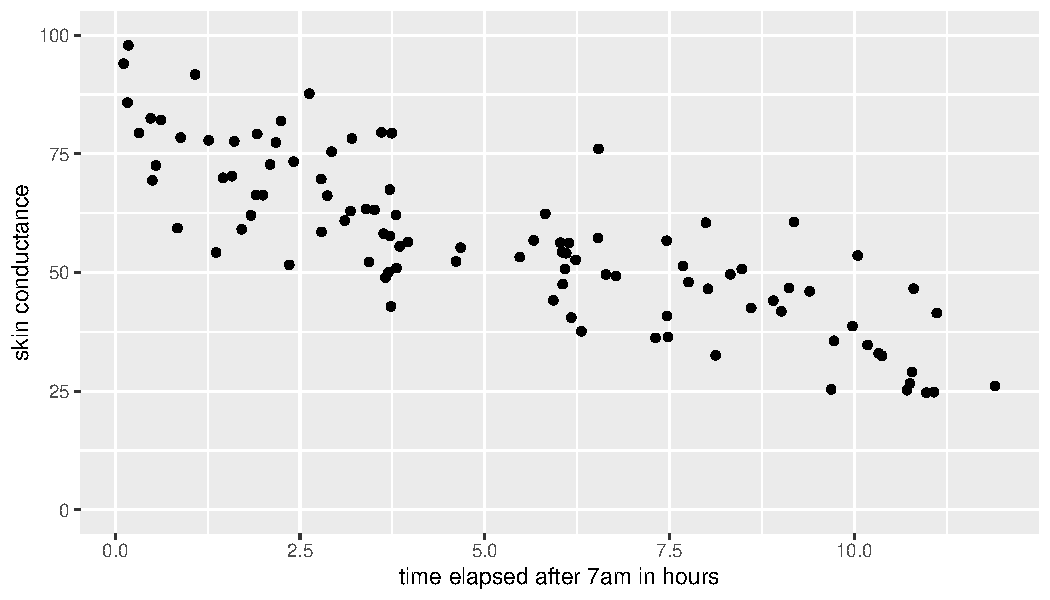
\includegraphics[width=\maxwidth]{figure/analysispremidpost7-1} 

}

\caption[Skin conductance measured in CEOs]{Skin conductance measured in CEOs.}\label{fig:analysispremidpost7}
\end{figure}


\end{knitrout}


\item What would the SPSS syntax look like? \\
\item If you got the output as in Figure \ref{fig:CEOexample}, what the predicted skin conductance be for a CEO at 15.00 hrs?


\begin{figure}[h]
    \begin{center}
       \includegraphics[scale=0.5]{/Users/stephanievandenberg/Dropbox/Statistiek_Onderwijs/Data" "Analysis/spss" "examples" "mixed" "linear" "model/pre-mid-post" "design/CEOexample.png}
    \end{center}
    \caption{Example output for the analysis of skin conductance in CEOs.}
    \label{fig:CEOexample}
\end{figure}


\item How much clustering is there for skin conductance across CEOs? \\
\item Would you say these individual differences are very important to take into account? \\
\item Is there a significant effect of time of day on skin conductance in CEOs?\\
\item What is the effect of time of day on skin conductance in CEOs? Also give the 95\% confidence interval of this effect.
\item Write a short paragraph that describes the results in APA format.
\item Suppose there is a new data set where every student's mood was tested at three points in time: During Christmas holidays (time point 1), during Easter holidays (time point 2) and at the start of the academic year, September 1 (time point 3). Look at the data plotted in Figure \ref{fig:analysispremidpost8}: do you think a linear effect is reasonable for this data set? Explain your answer.

\begin{knitrout}
\definecolor{shadecolor}{rgb}{0.969, 0.969, 0.969}\color{fgcolor}\begin{figure}

{\centering 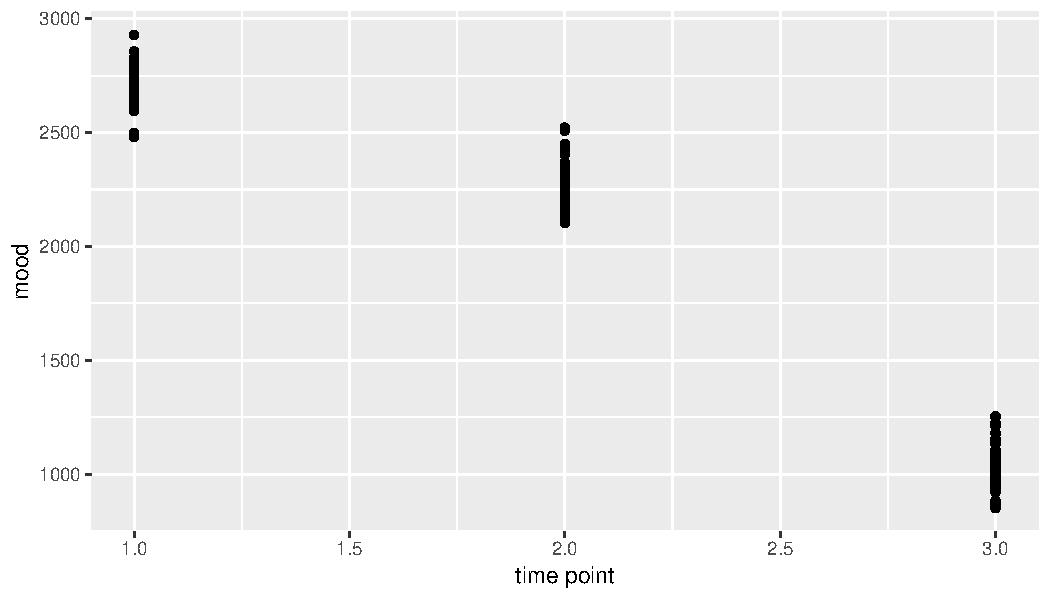
\includegraphics[width=\maxwidth]{figure/analysispremidpost8-1} 

}

\caption[Data on mood at three different time points]{Data on mood at three different time points.}\label{fig:analysispremidpost8}
\end{figure}


\end{knitrout}

\item Provide the syntax that you would use to analyze the problem of question 9.


\end{enumerate}

\subsection{Answers}


\begin{enumerate}

\item Yes, a general linear downward trend is observed for the skin conductance.
\item
\begin{verbatim}
MIXED conductance WITH time
  /FIXED=time
  /PRINT=DESCRIPTIVES  SOLUTION
  /RANDOM=intercept | SUBJECT(CEO) COVTYPE(VC).
\end{verbatim}
\item 15 hrs is equal to 8 hours after 7am, so the expected skin conductance is equal to $62 - 4 \times 8= 30$\\

\item The intraclass correlation coefficient is equal to $\frac{235}{235+247}=0.49$,
\item The correlation is quite different from 0, so there is certainly some clustering in the data and it is important to take these individual differences into account. \\
\item Yes, there is a signficant linear effect of time on skin conductance in CEOs, $t(59)=-4.24, p < 0.01$.\\
\item The linear effect of time of day on skin conductance in CEOs is around -4.13 points per hour after 7am (95 \% CI: -6.08 -- -2.18). \\
\item \begin{quotation}
        A linear mixed model was run with time as a quantitative predictor for skin conductance, including random effects for CEO. We found an effect of time of -4.13 points per hour which was significantly different from 0, $t(59)=-4.24, p < 0.001$. Therefore we conclude that time of day has an effect on skin conductance in the entire population of CEOs.
        \end{quotation}

\item The relationship is not linear: you cannot draw a straight line through the means of the three measurements.
\item Because we have multiple measurements from the same students we should use a MIXED analysis. Furthermore, a qualitave analysis would be more suitable, given the nonlinear relationship between time and mood. So we use the syntax:

\begin{verbatim}
MIXED mood BY time
  /FIXED=time
  /PRINT=DESCRIPTIVES  SOLUTION
  /RANDOM=intercept | SUBJECT(student) COVTYPE(VC).
\end{verbatim}

\end{enumerate}

\end{document}


